\mdfsetup{
%
frametitle={
%
\tikz[baseline=(current bounding box.east),
outer sep =0pt]
\node[anchor=east,rectangle,fill=red]
{\color{white} \small Nina \& Oma Lena};},
frametitleaboveskip=\dimexpr-\ht\strutbox\relax
}
\chapter*{\FontH{\Huge Nina und die rosa Delphine}}
\addcontentsline{toc}{chapter}{Nina und die rosa Delphine}
\begin{mdframed}[style=mystyle]
\lettrine[lines=3]{\color{red}H}{eute} war Oma Lena zu Besuch. Nina hatte sich schon lange auf sie gefreut. Oma Lena wohnte leider weit weg, in einem anderen Land und deswegen konnten sich die beiden nicht so oft sehen. Aber jetzt war es wieder so weit. 

Es war schon spät geworden, Geschenke mussten ja noch ausgepackt werden und dann Abendessen. Nina fand, dass Erwachsene immer viel zu viel Zeit mit Essen vergeuden. Anstatt stundenlang am Tisch zu sitzen, könnte man die Zeit doch viel besser nutzen. Sie würde das später mal anders machen, so viel war klar.

\enquote{Also gut} rief der Papa aus der Küche, \enquote{Oma darf dir noch eine Geschichte vorlesen. Aber nicht mehr so lange. Eine Viertelstunde, höchstens! Morgen ist wieder Kindergarten und dann musst du fit sein Nina.}

Nina seufzte. Als ob das heute wichtig wäre, dass sie morgen früh aufstehen muss. Ist doch mir egal. Oma Lena hatte ein Buch mitgebracht, das war das Geschenk gewesen. Von rosafarbenen Delphinen. Mama meinte, dass es die wirklich gäbe. Weit weg in einem Fluss namens Amazonas, der mitten durch einen Urwald fliesst. 

Nach dem Zähneputzen konnte nina endlich ins Bett springen und auf Oma warten. Nina überlegte, ob Mama ihr manchmal extra lange die Zähne putzte, um sie zu ärgern. Man könnte schon manchmal den Eindruck haben. Kater Fritz war auch gekommen, das war so seine Gewohnheit. Er sprang auf die Decke von Nina und wollte wohl auch zuhören. Fritz und Nina waren gute Freunde, obwohl er manchmal alleine mit Ninas Sachen spielte und die dann weg waren. Manchmal dauerte es Tage, bis die Sachen in irgendeiner Ecke wieder auftauchten. 

Oma klappte das Buch auf un blätterte ein bisschen zwischen den Seiten.

\enquote{Bis hierhin lese ich Dir heute vor, den Rest dann morgen. Einverstanden?} Oma tippte dazu auf eine Seite mit einem Bild eines Delphins. 

\enquote{Naaa gut.} antwortete Nina. Was sollte sie auch machen? Und erst einmal anfangen, der Rest findet sich später von alleine.
\end{mdframed}\medskip

Endlich legt sich der Sturm ein wenig. Fünf kleine rosafarbene Delphine treiben im offenen Meer. Das ist nichts Besonderes, sagt ihr? Doch, das ist es. Rosa Delphine müsst ihr wissen, leben eigentlich in einem grossen Fluss, der Amazonas heisst. Ins Meer gehören sie nicht! Wie sie da hingekommen sind? Das kam so.
\enquote{\it feliz cumpleanos a ti, 

feliz cumpleanos a ti

que los cumplas muy feliz

feliz cumpleanos a ti}

Das ist {\it Happy Birthday to you} auf Spanisch. Am Amzonas wird nämlich auch Spanisch gesprochen und heute hatte Rosa Geburtstag. Den Fünften. Rosa war ein Delphinkind, das in einem Nebenfluss eben jenes Amazonas lebt. Die Bäume am Rande des Flusses waren festlich geschmückt. Papageien hatten bunte Federn aufgehangen, Schmetterlinge schwirrten durch die Luft und die Affen waren in ausgelassener Feierlaune. Ein Ameisenbär steckte seinen Rüssel ins Wasser und machte Blasen, dass es nur so spritzte. Selbst das Faultier drehte seinen Kopf, um zu sehen, was da los ist. Und das musste was bedeuten, Rosa konnte sich nicht erinnern, überhaupt schon einmal gesehen zu haben, dass sich das Faultier bewegt.

Rosas Geburtstag war ein grosses Ereignis. Der fünfte Geburtstag ist nämlich bei Delphinen etwas ganz besonderes. Dann dürfen sie zum ersten Mal alleine aus dem Nebenfluss in den riesigen Amazonas schwimmen. Aufpassen, heisst es dann, denn es gibt viele Gefahren. Am gefährlichsten sind die Alligatoren. Wenn man da als kleiner Delphin nicht aufpasst, macht es Schnapp und weg ist man. Aber fünfjährige Delphine sind so gute Schwimmer, dass das eigentlich nie passiert. Auch vor Zitterallen muss man sich hüten. Wenn man die berührt, versetzen sie einem einen Stromschlag, der sehr weh tun kann. Onkel Konrad war das mal passiert, tagelang hatte er gejammert.

Rosa hatte natürlich ihre vier besten Freunde eingeladen. Es gab Fischkuchen, so wie ihn nur die Oma backen konnte. Rosas Freunde waren auch schon alle fünf, sie war die letzte. Sie hatten sich vorgenommen, den ersten Ausflug in den Amazonas gemeinsam zu machen.

Und dann ging es los. Rosas Mama hatte eine Träne im Auge, als sie ihr hinterher gewunken hatte, aber Unterwasser hat das natürlich niemand bemerkt. Rosa wusste es aber trotzdem. Aber es war Zeit, mit Fünf muss man das versuchen! Die erste Angst war schnell überwunden. Alle fünf Delphine musste eingestehen, so ein kleines Kribbeln im Bauch zu haben.

\enquote{Ach was, wir haben einfach nur zu viel Fischkuchen gegessen.} hiess es dann und weiter ging es. Plötzlich war ein risiger Schatten zu sehen. Rosa musste kurz aufschreien, aber es konnte schnell Entwarnung gegeben werden. Ein Arapaima schwamm träge durch das trübe Wassers. Arapaimas sind sehr grosse Fische. Im Amazonas sind nur Alligatoren und erwachsene Delphine noch grösser. Er brummte einen Gruss, Höflichkeit ist ausgesprochen wichtig im Amazonas, das gilt auch für alte knorzige Arapaimas.

\enquote{Ein Sturm zieht auf. Schwimmt zwischen die Mangrovenwurzeln, rate ich euch.} meinte er, ohne wirklich anzuhalten. 

Den fünf Freunden war das natürlich egal. Ein Sturm mag ärgerlich sein, wenn man an Land lebt, aber als Delphin im Wasser kann ja nichts passieren. Ob es noch regnet, ist ja dann egal. Und so tollten sie herum. Sie hatten sich schnell an ihre neue Freiheit gewöhnt. Niemand der da war und sagt, passt auf, da kommt ein Holzstamm geschwommen, oder nicht so den Schlamm aufwühlen und solche Sachen, die Erwachsene eben so zu Kindern sagen. Mit ihren Schwänzen wirbelten sie heute gemeinsam so viel Schlamm auf, dass das aussah wie ein Vulkanausbruch, wenn man vom Ufer zusah.

Das sich der Himmel immer mehr verdunkelt hatte, bemerkten sie gar nicht richtig. Der Wind frischte auf und wurde schnell immer stärker. Aus dem sanften Amazonas wurde eine wilde Welt aus Bergen und Tälern von Wasser. Der Urwald heisst in der Gegend hier nicht umsonst Regenwald. Erst spielten die fünf mit den Wellen, wurden aber schnell von ihnen mitgerissen.

Die gute Laune kippte schnell. Weder Rosa noch die anderen wussten sich zu helfen. Der Amazonas riss sie einfach mit, da half keine Anstrengung. Ach hätten sie nur auf den alten Arapaima gehört! Aber jetzt war das zu spät, jetzt mussten sie gegen das Wasser kämpfen. Ganze Bäume waren ausgreissen und schossen mit dem Amazonas mit. Da durfte man sich nicht in den Ästen verheddern und immer ausweichen. Der Sturm dauerte viele Stunden. Alle waren damit beschäftigt gewesen, Aufzupassen, nicht von den Wellen gegen irgendetwas geschleudert zu werden. Niemand hatte bemerkt, wo sie eigentlich hingespült wurden.

Der Sturm war zwar noch nicht vorbei, aber war etwas schwächer geworden. 

\enquote{Na prima} sagte Rosa. \enquote{Was für eine Geburtstagsfeier!}

Die Fünf sahen sich um, nichts, aber auch wirklich gar nichts war zu sehen. Nur Wasser, soweit das Auge reichte. Rosa versuchte es mit einem Sprung aus dem Wasser, um besser sehen zu können. Auch nichts. Kein Baum, kein Strauch, kein Vogel.

\enquote{Was ist mit dem Urwald passiert?} fragten sich die fünf Delphine gegenseitig. \enquote{Ist der vollständig überschwemmt? Gibt es keine Bäume mehr, ist jetzt alles Amazonas? Und warum schmeckt das Wasser hier so furchtbar?} 

Aber lange Zeit blieb ihnen nicht, noch bevor sie wirklich verzweifelt sein konnten, kam eine graues Dreieck auf sie zu. Erst bemerkte es niemand, aber als es immer schneller wurde, rief Rosa:

\enquote{Achtung, da kommt etwas!} Das graue Dreieck war die Rückenflosse eines grossen Fisches. Als er sein riesiges Maul aufriss, konnten sie drei Reihen sehr scharfer und spitzer Zähne sehen. Ein Hai? Von denen hatten die fünf schon gehört, aber die lebten doch im Meer? Waren sie etwa im Meer gelandet? Die Fünf schwammen um ihr Leben. Schnell in alle Richtungen wegschwimmen, um das Ungeheuer zu verwirren, dann wieder sammeln um sich nicht zu verlieren. 

Aber der Hai griff immer wieder an. Er kam auf die Fünf zugeschossen und riss sein furchtbares Maul auf. Jedesmal verfehlte er sie, aber immer etwas knapper. Viel Kraft immer wieder auszuweichen hatten sie nicht mehr. Alle hatten furchtbare Angst. Wieder blitzen die Zähne des Hais auf. Er raste auf Rosa zu. Die konnte sich vor Schreck und Erschöpfung nicht mehr bewegen. Wie versteinert blieb sie stehen. Plötzlich ein Schnattern, wie es nur Delphine können. Ein grosser blauer Delphin kam aus dem Wasser gesprungen und stupste den Hai in die Seite, so dass der abdrehen musste und verschwand. Aber er hatte Rosa noch an der Schwanzflosse erwischt. Nicht sehr schlimm, aber sie blutete ein bisschen und es tat furchtbar weh.

Ohne sich lange aufzuhalten meinte der: \enquote{Der Hai kommt gleich zurück. Kommt mit mir mit, schnell! Alle nochmals gut Luft holen und los!}

Alle atmeten tief ein und tauchten hinter dem blauen Delphin her. Tiefer und immer tiefer tauchte der. So tief, wie der Amazonas an keiner Stelle war, tief, wie das nur im Meer geht. Ihr wisst ja, dass Delphine nicht wie Fische unterwasser atmen können, sondern immer an die Oberfläche kommen müssen. Alle hatten das Gefühl, es nie wieder bis an die Oberfläche zu schaffen, so lange hatten sie jetzt schon die Luft angehalten. Aber es ging immer weiter und weiter. Sie tauchten an einer Felswand entlang und fanden den gut versteckten Eingang zu einer Höhle. Dort schwammen sie hinein und konnten auch wieder Luft holen. Eine Höhle unter dem Meer, in der es sogar Luft gab. Von weit weg drang sogar etwas Licht herein.

Die fünf Freunde mussten hächeln. Keiner von ihnen hatte schon jemals so lange die Luft angehalten.Es war eigenartig still hier drinnen.

\enquote{Ist jemand verletzt?} fragte der blaue Delphin. Nur Rosa hatte eine schwere Schramme abbekommen, den anderen ging es gut, aber es waren alle sehr erschöpft.

\enquote{Das heilt wieder.} meinte der blaue Delphin, nachdem er sich die Wunde angesehen hatte. \enquote{Ihr bleibt hier und ich hole uns erst einmal ein paar Fische.}

Ohne ein Wort zu reden schlangen die fünf Freunde die Fische herunter. So langsam kehrte auch ihre Kraft zurück. Sie mussten dem blauen Delphin ganz genau erklären, was passiert war.

Der wiegte den Kopf hin un her und meinte, dass der Sturm sie wohl ins offene Meer getragen hatte. Sie sollten sich keine sorgen machen, es würde alles wieder gut werden. Abwarten, bis der Sturm vorbei ist und der Hai die Suche aufgegeben hätte und dann würde er ihnen den Weg zurück zeigen.

Aber das war leichter gesagt als getan. Rosa konnte mit ihrer verletzten Flosse unmöglich nochmals so lange tauchen. Und es würde mindestens zwei Wochen dauern, bis sie wieder gesund war. Und weil ihr Kopf aus dem Wasser guckte, konnte man ausnahmsweise sehen, wie einem Delphin grosse Tränen aus den Augen kamen.


\begin{mdframed}[style=mystyle]
Sie waren auf der Seite mit dem Delphinbild angekommen. Oma klappte das Buch zu und gab Nina einen Kuss auf die Stirn.

\enquote{Schlaf gut mein Engel.} sagte sie \enquote{Und morgen, gleich wen nDu aus dem Kindergarten zurück bist, lese ich Dir den Rest der Geschichte vor.} Selbstverständlich protestierte Nina. Wie kann man nur so gemein sein und aufhören, wen nes am spannendsten ist! Das war jetzt schon das zweite Mal an diese mAbend, dass sie sich vornehmen musste, es später, wenn sie selbst gross sein würde, besser zu machen. Aber noch bevor sie Oma eine Standpauke halten konnte, musste sie so fest gähnen, dass sie beschloss, auf lauten Protest zu verzichten. Dann eben morgen weiter.

Kater Fritz wurde aus dem Zimemr gescheucht, die Tür blieb einen Spalt offen und dann schlief Nina sofort ein.

Am nächsten Morgen konnte es Nina kaum abwarten, wie die Geschichte wohl weiterging. Die arme Rosa! Wie sie wohl wieder aus der Hhle kommen würde? Nina kontrollierte nochmals, dass das Buch auch so lag, dass Oma es gleich nehmen konnte, wen nsie zurück vom Kindergarten kam. Sie hatte so lange bei Mama gequängelt, bis diese versprochen hatte, dass es das Mittag erst gibt, wen ndie Geschichte zu Ende erzählt war.

Endlich war es weit. Ohne wie sonst auf ihre Freundinnen zu warten, rannte Nina nach Hause. Oma sass schon lachend auf der Couch und meinte, Nina solle das Buch holen, es könne gleich los gehen.

Aber das Buch war nicht mehr da! Weg!

\enquote{Maaaaamaaaa, Maaaaaaaaamaaaaa! Wo hast du das Delphin-Buch hingemacht?} Nina war ausser sich. Schweren Schrittes kam Mama die Treppe hinauf.

\enquote{Ich hab dein Buch nicht, Schatz. Wo hast du es denn hingelegt?} Auf so eine Frage antwortete Nina gar nicht erst. Als ob sie da nicht als allererstes gesucht hätte. Verzweifelt riss sie alle Bücher aus dem Büchergestell, aber das Delphin-Buch war nicht dabei.

Nach einem kleinen Streit mit Mama, die nicht begriff, wie Ernst die Lage war und nur die zugegebenermassen schlimme Unordnung kritisierte, musste Nina weinen. Das Buch war weg, wie vom Erdboden verschluckt. Oma kam jetzt auch hoch und wollte wissen, was los sei. Das Mama immer noch schimpfte wegen der vielen verstreuten Bücher, merkte Nina gar nicht richtig. Oma konnte schlichten. Gemeinsam räumten die Drei die Bücher wieder auf und überlegten, wo das Buch wohl sein könne.

Mama hatte die Lösung. Fritz! Es konnte nur Kater Fritz gewesen sein. Wie ein Pfeil schoss Nina die Treppe herunter und schimpfte auf Fritz ein. Der aber gähnte nur und wollte gekrault werden. Wirklich böse kontne Nina ihm ja nicht sein, der wollte ja auch nur spielen.

Oma streichelte Nina am Abend über den Kopf. Sie sagte:

\enquote{Manchmal braucht man gar keine Bücher, um Geschichten zu erzählen. Es ist ja nur das Buch weg, aber die Geschichte ist noch da. Du machst jetzt die Augen zu und konzentrierst dich ganz fest auf Rosa. Du musst ganz sehr an sie denken und dann wirst du schon sehen\dots}

Wieder bekam Nina einen Kuss, zog die Decke über den Kopf und dachte an Rosa. Sie erzählte sich nochmals selbst die Geschichte, soweit sie sich an gestern Abend erinnern konnte.
\end{mdframed}\medskip

Plötzlich war auch Nina in der Höhle unter dem Meer. Sie hatte den Koffer mit ihren Lieblingsspielsachen mit und sass auf einem Stein. Um sie herum schwappte das Meer gegen den Stein. genau Rosa bemerkte auch sie als erstes diese Stille. Und das Licht von oben. Es war nicht zu erkennen, wo es herkam, aber es musste eine Höhle unter einer Insel sein.

Nina hatte keine Angst. Sie wusste, dass es nur ein Traum war und ihr nichts passieren konnte. Wen nman träumt musste man nur ganz laut {\it Gefälligst aufwachen!} schreien, dann war der Traum sofort vorbei. Zur Sicherheit kniff sie sich in den Arm. Den Trick hatte ihr mal ihre Cousine gezeigt. Die war schon drei Jahre älter und wusste daher alles. Wenn man sich kneift und etwas spürt, is talles in Ordnung. Wenn man nichts spürt, träumt man hatte die erklärt. und tatsächlich. Nina spürte nichts.






\begin{figure}[hb]
\centering
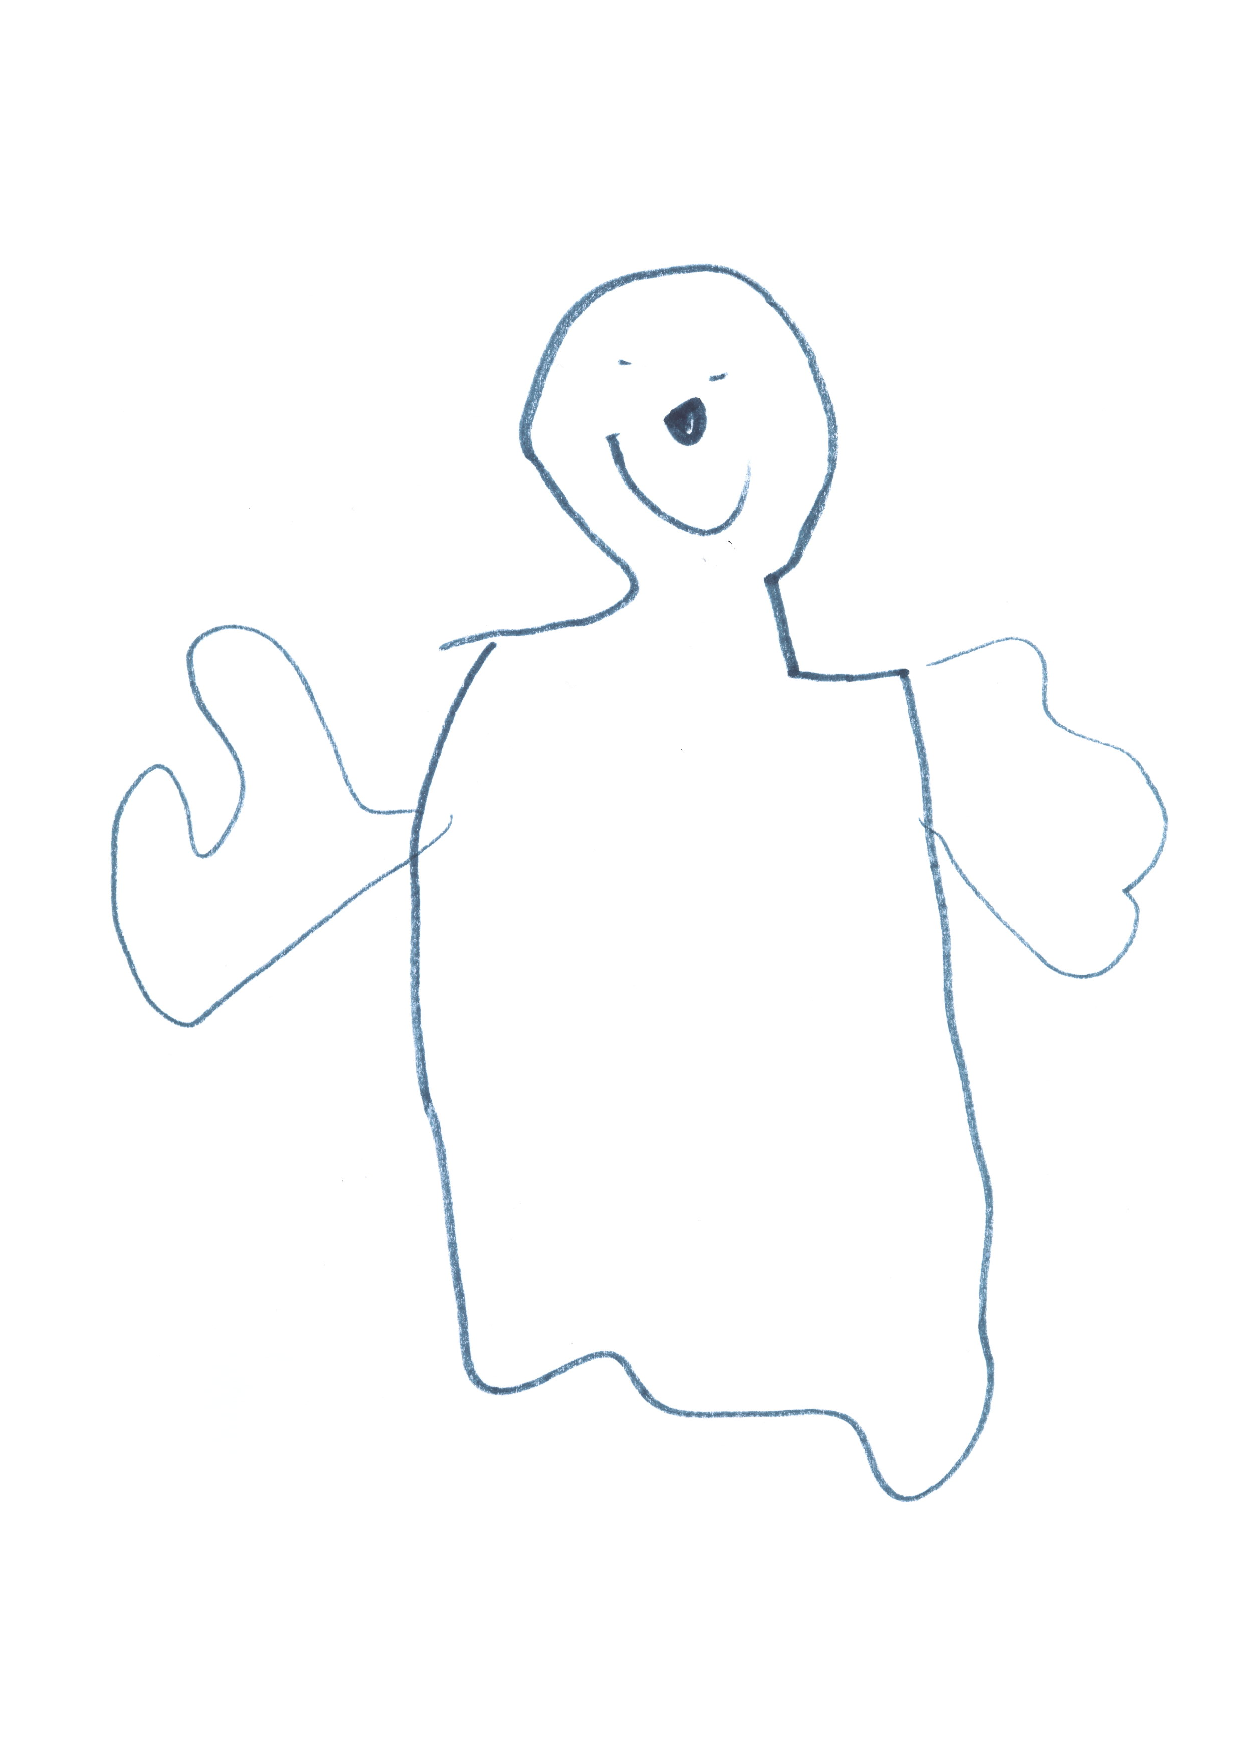
\includegraphics[width=.7\textwidth]{bilder/gespenst1.pdf}
\end{figure}

\begin{mdframed}[style=mystyle]
\end{mdframed}\medskip
